\subsection{State-Machine-basierte Programmierung}\label{subsec:fsmprogrammierung}
\begin{quote}
    ''\textit{Have you tried turning it off and on again?}''  \\ -- Ein Jeder, der die Macht von \acp{FSM} verstanden hat.
\end{quote}

Bis zum jetzigen Zeitpunkt kann man den beschriebenen \ac{DBP}-Ansatz mit dem von SAM Labs (Kapitel \ref{subsubsec:samlabs}) vergleichen, auch mit seinen Problem (''Sequentiell contra Parallel'' und ''Signalpriorisierung''). Wie schon in den Problemen beschrieben müssen es Aktoren möglich sein mit parallel eintreffenden Signalen umgehen können, um Szenarien wie die in S\#2 beschriebene Ampelschaltung und die in S\#3 beschriebene Vermeidung von Signalkonflikten zu ermöglichen.

Die einzige Möglichkeit für SAM Labs diesen Problemen aus dem Weg zu gehen ist es, sequentielle Logik mit der Datenfluss-Logik zu vermischen. Dies geschieht indem die Steuerungslogik der Aktoren auf der selben Ebene deklariert werden, wie die Logik, die Signale in eine nutzbare Form transformieren. In flowws wird einen anderen Weg gegangen. Es kommt eine Paradigma zum Steuern der Aktoren, welches weite Verbreitung in der IT und in \textit{Embedded Hardware} genießt: die \acl{FSM} (engl. endlicher Zustandsautomat).


\begin{figure}[h]
  \centering
  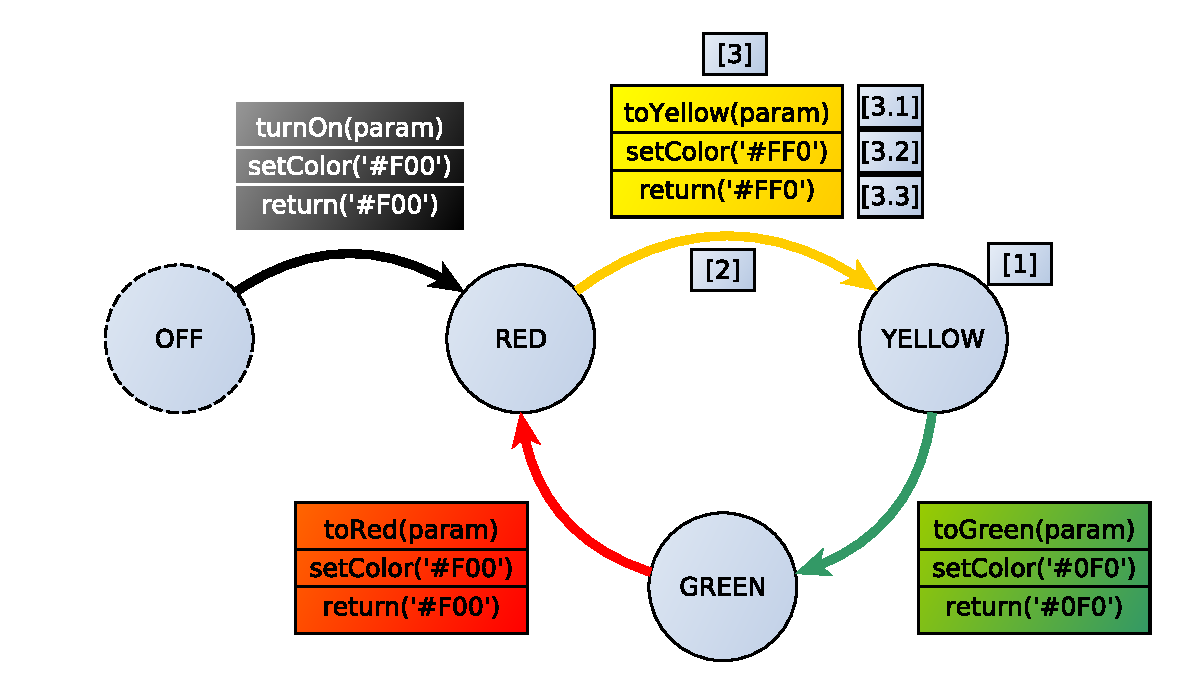
\includegraphics[width=0.85\textwidth]{bilder/chapter4/chapter4_2/beispielstatemachine.pdf}
  \caption{Die \ac{FSM} eines cBlocks mit LED-Aktor. Es existieren vier Zustände: OFF (Startzustand), RED, YELLOW, GREEN; und vier Übergänge: turnOn(), toYellow(), toGreen() und toRed(). Jeder der Übergänge verwendet in diesem Fall die setColor()-Funktion des LED-Aktors um die LED in der jeweils definierten Farbe wechseln. Jeder Übergang nimmt die Parameter (param) entgegen, was dem \textit{Payload} eines \textit{Events} entspricht. Dieser wird in diesem Beispiel entgegen genommen aber nicht verwendet. Zusätzlich erzeugt jeder Übergang mit return(<farbcode>) ein weiteres Event.}
  \label{fig:beispielfsm}
\end{figure}
 
\acp{FSM} sind Systeme von einer endlichen Menge von Zuständen (engl. \textit{States}), die auf eine endliche Menge von Ereignissen (engtl. \textit{Events}) reagieren, welche außerhalb des Systems auftreten und auf das System einwirken. Die Reaktion einer \ac{FSM} auf eintreffende Signale werden abhängig einer endlichen Anzahl von Übergängen (engl. \textit{Transitions}) gesteuert. Kann eine \ac{FSM} zu jeder Zeit nur einen Zustand annehmen ist sie \textit{deterministisch} (\cite{hopcroft2013introduction}). 

Die Parallelen zu cBlocks bzw. flowws werden hierbei klar: cBlocks-Aktoren können als \acp{FSM} dargestellt werden. Ein Beispiel ist in Abbildung \ref{fig:beispielfsm} in Form eines LED-cBlocks gegeben, der eine Ampelschaltung modelliert. Es sind hierbei vier Elemente sichtbar, welche im Domänen-Modell (Abbildung \ref{fig:domainmodelfsm}) korrespondieren:
\begin{itemize}
    \item \textbf{Zustände/States [1]:} Ein Zustand drückt wie klassischen \ac{FSM}-Modell den momentanen Status eines Automaten bzw. des Aktor-cBlocks aus. Diese Status ist nicht an die Ausprägung eines bestimmten Eigenschaft des Aktors gebunden, sprich ''RED'' bedeutet nicht zwangsweise die Farbe Rot. Vielmehr legt ein Zustand fest, welche zukünftigen Zustände beim eintreffen des nächsten Ereignisses erreichbar sind. In Abbildung \ref{fig:beispielfsm} ist es bspw. nicht möglich von Status ''RED'' in ''GREEN'' direkt zu springen. Durch dieses Konstrukt lässt sich sequentielles Verhalten in den cBlock einprogrammieren. Zusätzlich existiert ein Anfangszustand, der die initiale Ausprägungen des cBlock-Aktors definiert.
    \item \textbf{Übergänge/Transitions [2]:} Die Übergänge werden wie die Zustände durch den Nutzer definiert. Sie verbinden die einzelnen Zustände und ermöglichen somit das modellieren des Verhaltens eines cBlocks. Dadurch gestatten bzw. verbieten Übergänge durch ihre Existenz bzw. Abwesenheit eine Signalpriorisierung vorzunehmen. Eine \ac{FSM} erlaubt es die Logik des cBlocks graphisch so zu modellieren, dass ein (zum momentanen Status) im Konflikt stehendes eintreffendes Signal ignoriert werden kann.
    \item \textbf{Übergangslogik/Transitional Logic [3]:} Die Logik, welche die Eigenschaften eines Aktor-cBlocks manipuliert und somit physikalische Signale erzeugt ist innerhalb der Übergänge. Sie besteht im Grunde aus drei Teilen:
    \begin{itemize}
        \item Die \textbf{Deklaration [3.1]} gibt den Namen des Ereignisses an, welches den Übergang hervorruft. Wird der Aktor als \textit{Black Box} dargestellt ist dies eine Eingabeschnittstelle, die nach Außen sichtbar ist. Der Parameter in der Deklaration symbolisiert den Payload, des eintreffenden Events und kann optional von der Funktionslogik weiterverarbeitet werden.
        \item Die \textbf{Funktionslogik [3.2]} beinhaltet die konkreten Instruktionen, die die Eigenschaften des cBlocks manipulieren. In Abbildung \ref{fig:beispielfsm} wird beispielsweise \texttt{setColor(<farbe>)} verwendet um die Farbe der LED zu ändern. Diese Funktionen sind für jeden Aktor speziell und werden vom cBlocks \textit{Back-End} vorgegeben. Experten wie Persona Mark können allerdings weitere Funktionen hinzufügen und somit den Funktionsumfang eines Aktors für Laura erweitern.
        \item Der \textbf{Rückgabewert [3.3]} ist optional und gibt ähnlich wie die Deklaration, eine Schnittstelle der \textit{Black Box} an. In diesem Fall allerdings eine Output-Schnittstelle. Durch diese Schnittstellen kann ein Aktor seine Zustandsänderung dem Rest des Systems mitteilen und somit neue digitale Signale erzeugen. 
    \end{itemize}
\end{itemize}

\begin{figure}[h]
  \centering
  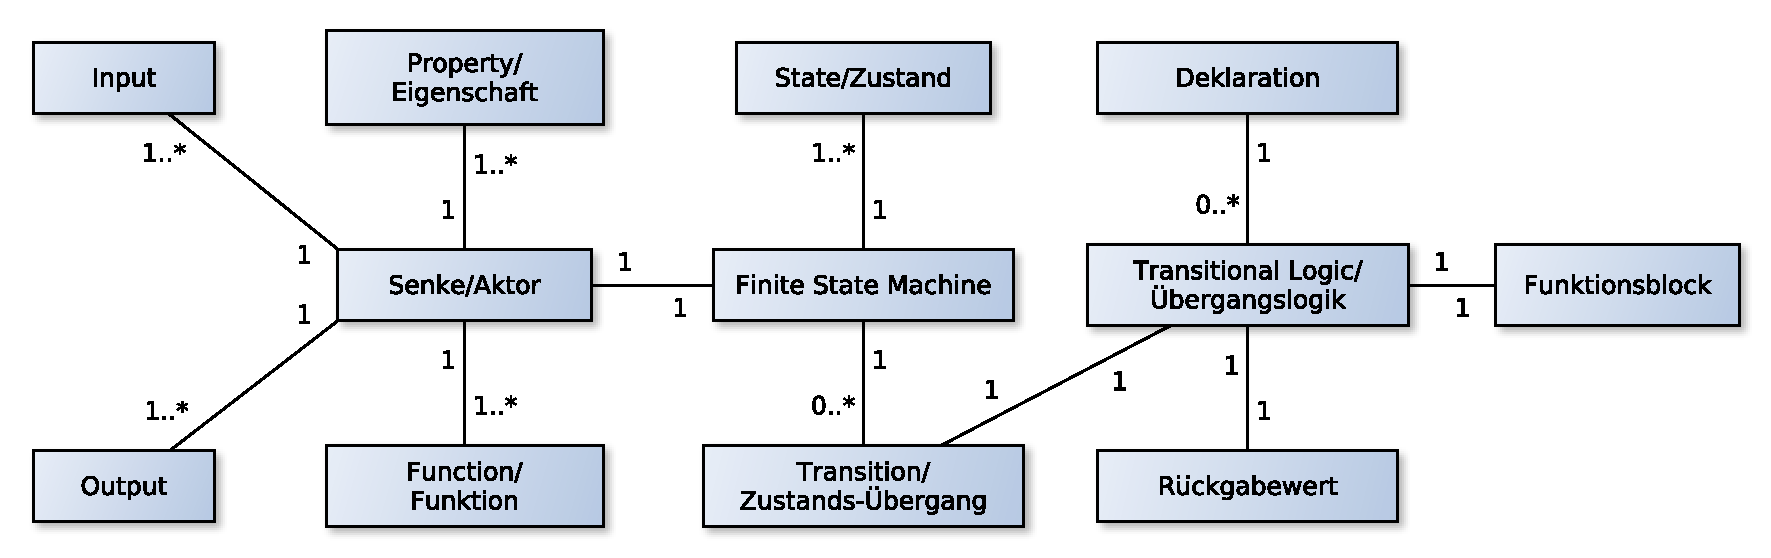
\includegraphics[width=1\textwidth]{bilder/chapter4/chapter4_2/domainmodellaktor.pdf}
  \caption{Das Domänenmodell des Aktors bzw. der \ac{FSM} ist eine Detailansicht von Abbildung \ref{fig:bfddomainmodel} hinsichtlich der Bestandteile des Aktors. }
  \label{fig:domainmodelfsm}
\end{figure}

Durch das Verwenden einer \ac{FSM} ergeben sich mehrere Vorteile. Durch gute Visualisierungsmöglichkeit der \ac{FSM} und der weiten Verbreitung des Modells kann die Erlernbarkeit gefördert und somit NFN\#2, adressiert werden. Zusätzlich erlaubt das Benutzen von \ac{FSM}, wie in  NFN\#0 gefordert, sequentielles Verhalten zu modellieren, indem es die asynchronen Ereignisse, die auf den Aktor-cBlock einwirken, sequentiell zu verarbeiten. Das Hinzufügen von zusätzlichen Aktor-Funktionen durch Experten, kann das System nachträglich erweitert werden, wie es von NFN\#5 verlangt ist. Im nächsten Schritt muss geklärt werden, wie \ac{DBP} und \ac{FSM} miteinander integriert werden, um Endnutzern das Entwickeln von Programmen innerhalb von flowws zu ermöglichen.